\part{Analytic theory of partitions}\label{part3} %%% part III

\chapter{Lecture}\label{part3:lec16} %%% 16
\markboth{\thechapter. Lecture}{\thechapter. Lecture}

Our\pageoriginale aim will be now to get an explicit formula for
$p(n)$ and things connected with it. Later we shall return to the
function $\eta (\tau)$ and the discussion of the sign of the square
root. That will again lead us into some aspects of the theory of
$\mathscr{V}$-functions connected with quadratic residues. 

Let us come to our topic. Euler had, as we know, the identity:
$$
\sum^\infty_{n=0} p(n) x^n = \frac{1}{\prod\limits^\infty_{m=1} (1-x^m)}.
$$

This is the starting point of the function-theoretic treatment of
$p(n)$. 
$$
p(n)= \frac{1}{2 \pi i} \int_c \frac{f(x)}{x^{n+1}} dx,
$$
where $f(x) = \prod\limits^\infty_{m=1} (1-x^m)^{-1}$ and $C$ is a
suitable closed path contained in the unit circle, in which the
function is analytic, and enclosing the origin. Since $\sum p(n) x^n$
is a power series beginning with 1, this means a little more. $n$ may
be negative also; and when $n$ is negative $f(x) x^{-n-1}$ is regular
at $x=0$. Therefore we include negative exponents also in our
discussion; we put $p(-n) =0$, $n> 0$, when is convenient. Hereafter
we shall take $n$ to be an integer $\gtreqless 0$; we shall choose $n$
and keep it fixed throughout our discussion.

It\pageoriginale is a little more comfortable to change the variable
and put $x= e^{2 \pi i \tau}$, $\im \tau > 0$, which is familiar to us.

$dx= e^{2 \pi i \tau}\cdot 2 \pi i d \tau$ and the whole thing boils
down to 
$$
p(n) = \int_\alpha^{\alpha+1} f(e^{2 \pi i \tau}) e^{- 2 \pi i n \tau}
d \tau
$$
\begin{figure}[H]
  \centering{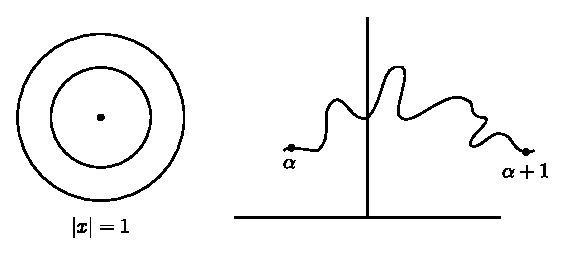
\includegraphics{vol2-figures/fig2.21.eps}}
\end{figure}

It is enough to take the integral along a path from an arbitrary point
$\alpha$ to the point $\alpha+1$, because the integrand is periodic,
with period 1. (This path replaces the original path $C$ that we had
in the $x$-plane before we changed the variable). The method of Hardy
and Ramanujan was to take a curve rather close to the unit circle
which is a natural boundary for the function (this will come out in
the course of the argument). They cut up the path of integration into
pieces called Farey arcs, and the trick was to replace the function by
a simpler approximating function on each specific Farey arc. We shall
use not exactly this method, but consider a special path from $\alpha$
to $\alpha +1$, which we shall discuss.

We shall keep our formula in abeyance for a moment and give a short
discussion of Farey  series (`series' here is not to be understood in
the sense of infinite series, but as just an aggregate of
numbers). Cauchy\pageoriginale did make all the observation
attributed by Hardy and Wright to Farey; Farey made his remarks in the
Philosophical Magazine, 1816. He put only questions; Cauchy had all
the answers earlier.

We deal with the interval $(0, 1)$. Choose all reduced fractions whose
denominators do not exceed $1, 2, 3, \cdots $ in succession. Let us
write down the first few, with the fractions arranged in increasing
order of magnitude. 

\medskip
\noindent 
\tabcolsep=7pt
\begin{tabular}{cccccccccccccc}
 &&&&$\frac{0}{1}$&&&&$\frac{1}{1}$&&&&& order 1\\
 &&&$\frac{0}{1}$&&&$\frac{1}{2}$&&&$\frac{1}{1}$&&&& order 2\\
 &&$\frac{0}{1}$ &&$\frac{1}{3}$& &$\frac{1}{2}$& &$\frac{2}{3}$&
  &$\frac{1}{1}$  &&& order 3\\
 &$\frac{0}{1}$& &$\frac{1}{4}$&$\frac{1}{3}$& &$\frac{1}{2}$&
  &$\frac{2}{3}$ & $\frac{3}{4}$ & &$\frac{1}{1}$ & &order 4\\
 $\frac{0}{1}$ & &$\frac{1}{5}$ & $\frac{1}{4}$& $\frac{1}{3}$&
  $\frac{2}{5}$ & $\frac{1}{2}$ &$\frac{3}{5}$ &$\frac{2}{3}$
  &$\frac{3}{4}$ & $\frac{4}{5}$& &$\frac{1}{1}$& order 5
\end{tabular}
\medskip

The interesting fact is that we can write down a new in the following
way. We repeat the old row and introduce some new fractions. If
$\dfrac{h}{k} < \dfrac{h'}{k'}$ are adjacent fractions in a row, the
new one introduced between these in the next row is
$\dfrac{h+h'}{k+k'}$, provided that the denominator is of the proper
size. Following Hardy and Littlewood we call $\dfrac{h+h'}{k+k'}$ the
`mediant' between $\dfrac{h}{k}$ and $\dfrac{h'}{k'}$. We have
$\dfrac{h}{k} < \dfrac{h+h'}{k+k'} < \dfrac{h'}{k'}$, so that the
order is automatically the natural order. We call that row which has
denominator $k \leq N$, the \textit{Farey series of order $N$}. We get
this by forming mediants from the preceding row. Farey made the
following observation. Take two adjacent fractions in a row; then the
determinant formed by their numerators and denominators is equal to
$-1$. For instance, in the fifth row $\dfrac{1}{3}$ and $\dfrac{2}{5}$
are adjacent and $\begin{vmatrix} 1 & 2\\ 3 &
5 \end{vmatrix}=-1$***********. If we now prove that
new\pageoriginale fractions are always obtained by using mediants,
then we can be sure, by induction, that this determinant is always
$-1$. For, let
\begin{align*}
  \begin{vmatrix}
    h & h'\\
    k & k'
  \end{vmatrix} & = - 1; ~\text{then}~\\
  \begin{vmatrix}
    h & h+h'\\
    k & k+k'
  \end{vmatrix} & =- 1=  
  \begin{vmatrix} h+h' & h'\\ k+k' & k'  \end{vmatrix} 
\end{align*}

If indeed only mediants occur, Farey's observation is justified. And
this is so. Observe that these fractions must all appear in their
lowest terms; otherwise, the common factor will show up and the
determinant would not be $-1$. Suppose that we want to find out where
a particular fraction appears. Say, we have in mind a specific
fraction $\dfrac{H}{K}$. It should occur for the first time in the
Farey series of order $N=K$ and it should not be present on any series
of order $< K$. Now look at $N=K-1$ where $\dfrac{H}{K}$ is not
present. If we put it in, it will belong somewhere according to its
size, i.e., we can find fractions $\dfrac{h_1}{k_1},
\dfrac{h_2}{k_2}$, with $k, k_2 < N$ such that $\dfrac{h_1}{k_1} <
\dfrac{H}{K} < \dfrac{h_2}{k_2}$. Assume that the determinant property
and the mediant property are true for order $N< K$. (They are clearly
true up to order 5, as we verify by inspection, so that we can start
induction). Now prove them for $N=K$. Try to determine $H$ and $K$ by
interpolation between $\dfrac{h_1}{k_1}$ and $\dfrac{h_2}{k_2}$. Put
\begin{align*}
  Hk_1 - Kh_1  & = \lambda,\\
  - Hk_2 + Kh_2 & = \mu,
\end{align*}
so that $\lambda$ and $\mu$ are integers $>0$. Solving for $H$ and $K$
by Cramer's\pageoriginale rule,
$$
H= \frac{\begin{vmatrix} \lambda & -h_1\\ \mu & h_2 \end{vmatrix}}{
  \begin{vmatrix} h_2 & k_2\\ h_1 & k_1 \end{vmatrix}}, \quad K=
  \frac{\begin{vmatrix} \lambda & -k_1\\ \mu & k_2 \end{vmatrix}}{
    \begin{vmatrix} h_2 & k_2\\ h_1 & k_1 \end{vmatrix}}
$$

By induction hypothesis, the denominator $=1$, and so
\begin{align*}
  H & = \lambda h_2 + \mu h_1\\
  K & = \lambda k_2 + \mu k_1\\
  \text{or} \qquad \frac{H}{K} & = \frac{\lambda h_2 + \mu
    h_1}{\lambda k_2+ \mu k_1}.\qquad 
\end{align*}

What do we know about $K$? $K$ did not appear in a series of order
$K-1$; $k_1$ and $k_2$ are clearly less than $K$. What we have found
out so far is that any fraction lying between $\dfrac{h_1}{k_1}$ and
$\dfrac{h_2}{k_2}$ can be put in the form $\dfrac{\lambda h_2 + \mu
  h_1}{\lambda k_2 + \mu k_1}$. Of these only one interests us - that
one with lowest denominator. This comes after the ones used so
far. Look for the one with lowest denominator; this corresponds to the
smallest possible $\lambda, \mu$, i.e., $\lambda= \mu =1$. Hence first
among the many later appearing ones is $\dfrac{H}{K}= \dfrac{h_1 +
  h_2}{k_1+ k_2}$, i.e., if in the next Farey series a new fraction is
called for, that is produced by a mediant. So what was true for $K-1$
is true for $K$; and the thing runs on.

One remark is interesting, which was used in the Hardy - Littlewood-
Ramanujan discussion. In the Farey series of order $N$, let
$\dfrac{h_1}{k_1}$ and $\dfrac{h_2}{k_2}$ be adjacent
fractions. $\dfrac{h_1}{k_1} < \dfrac{h_2}{k_2} \cdot
\dfrac{h_1+h_2}{k_1+ k_2}$ does not being these. It is of higher
order. This says that $k_1 + k_2 > N$. For two
adjacent\pageoriginale fractions in the Farey series of order $N$,
the sum of the denominators exceeds $N$. Both $k_1$ and $k_2 \leq N$,
so 
$$
2N \geq k_1+k_2 > N.
$$  

$k_1$ and $k_2$ are equal only in the first row, otherwise it would
ruin the determinant rule. So
$$
2N > k_1 + k_2 > N, N>1.
$$

This was very often used in the Hardy - Ramanujan discussion. (The
Farey series is an interesting way to start number theory with. We can
derive from it Euclid's lemma of decomposition of an integer into
primes. This is a concrete way of doing elementary number theory). 

We now come to the special path of integration. For this we use
\textit{Ford Circles} (L.R. Ford, American Mathematical Monthly, 45
(1938), 568-601). We describe a series of circles in the upper
half-plane. To each proper fraction $\dfrac{h}{k}$ we associate a
circle $C_{hk}$ with centre $\tau_{hk} = \dfrac{h}{k} +
\dfrac{i}{2k^2}$ and radius $\dfrac{1}{2k^2}$, so the circles all
touch the real axis. 
\begin{figure}[H]
  \centering{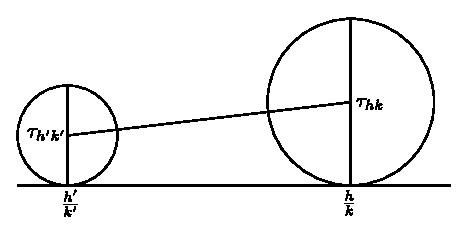
\includegraphics{vol2-figures/fig2.22.eps}}
\end{figure}

Take another Ford circle $C_{h'k'}$, with centre at
$\tau_{h'k'}$. Calculate the distance between the centres.
$$
\left| \tau_{hk}- \tau_{h'k'} \right|^2= \left( \frac{h}{k}-
\frac{h'}{k'}\right)^2 + \left( \frac{1}{2k^2} - \frac{1}{2k'^2}\right)^2.
$$

The \pageoriginale sum of the radii $= \frac{1}{2 k^2} +
\frac{1}{2k'^2}$
\begin{align*}
  \left| \tau_{hk} - \tau_{h' k'} \right|^2 - \left( \frac{1}{2k^2} +
  \frac{1}{2k'^2} \right) & = \left( \frac{h}{k}-
  \frac{h'}{k'}\right)^2 - \frac{1}{k^2 h'^2}\\
  & = \frac{(h k' - h' k)^2-1}{k^2 k'^2} \geq 0,
\end{align*}
since $h$, $k$ are coprime and so $\left|\begin{smallmatrix} h &
k\\ h' & k'\end{smallmatrix}\right|$ is an integer $\neq 0$. So two
Ford circles never intersect. And they touch if and only if 
$$
\begin{vmatrix}
  h & k\\
  h' & k'
\end{vmatrix}= \pm 1,
$$
i.e., if in a Farey series $\dfrac{h}{k}, \dfrac{h'}{k'}$ have
appeared as adjacent fractions. 

Now we come to the description of the path of integration from
$\alpha$ to $\alpha + 1$. For this consider the Ford circle $C_{hk}$. 

\begin{figure}[H]
  \centering{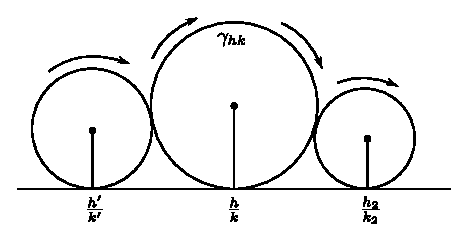
\includegraphics{vol2-figures/fig2.23.eps}}
\end{figure}
In a certain Farey series of order $N$ we have adjacent fractions
$\dfrac{h_1}{k_1}< \dfrac{h}{k}< \dfrac{h_2}{k_2}$. (We know exactly
which are adjacent ones in a\pageoriginale specific series). Draw
also the Ford circles $C_{h_1 k_1}$ and $C_{h_2 k_2}$. These touch
$C_{hk}$. Take the arc $\gamma_{hk}$ of $C_{hk}$ from one point of
contact to the other in the clockwise sense (the arc chosen is the one
not touching the real axis). This we do for all Farey fractions of a
given order. We call the path belonging to Farey series of order $N
~P_N$. Let us describe this in a few cases. 

We fix $\alpha=i$ and pass to $\alpha + 1= i +1$. Take $N=1$; we have
two circles of radii 2 each with centres at $\dfrac{i}{2}$ and
$1+\dfrac{i}{2}$ 

\begin{figure}[H]
  \centering{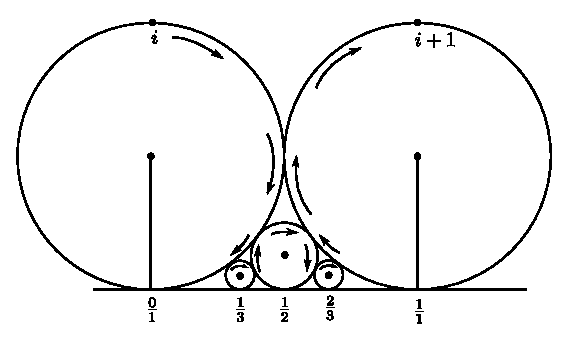
\includegraphics{vol2-figures/fig2.24.eps}}
\end{figure}
$\rho_1$ will be the path consisting of arcs from $i$ to $\frac{1}{2}
+ \frac{i}{2}$ and $\frac{1}{2} + \frac{i}{2}$ to $i+1$. Later because
of the periodicity of $f(e^{2\pi i \tau})$ we shall replace the second
piece by the arc from $- \frac{1}{2} + \frac{i}{2}$ to $i$. Next
consider Farey series of order 2; $\dfrac{0}{1}$ and $\dfrac{1}{1}$
are no longer adjacent. The path now comprises the arc of $C_{01}$
from $i$ to the point of contact with $C_{12}$, the arc of $C_{12}$
from this point to\pageoriginale the point of contact with $C_{11}$
and the arc of $C_{11}$ from this point to $i+1$. Similarly at the
next stage we pass from $i$ on $C_{01}$ to $i+1$ on $C_{11}$ through
the appropriate arcs on the circles $C_{13}$, $C_{12}$, $C_{23}$ in
order. So the old arcs are always retained but get extended and new
arcs spring into being and the path gets longer and longer. At no
stage does the path intersect itself, but these are points of
contact. The path is complicated and was not invented in one
sitting. The Farey dissection of Hardy and Ramanujan can be pictured
as composed of segments parallel to the imaginary axis. Here it is more
complicated. 

We need a few things for our consideration. We want the point of
contact of $C_{hk}$ and $C_{h' k'}$. This is easily seen to be the
point 
\begin{align*}
  \tau_{hk} \frac{\frac{1}{2k'^2}}{\frac{1}{2k^2}+ \frac{1}{2k'^2}} +
  \tau_{h'k'} \frac{\frac{1}{2k^2}}{\frac{1}{2k^2} + \frac{1}{2k'2}} &
  =
  \left( \frac{h}{k} + \frac{i}{2k^2}\right) \frac{k^2}{k^2+ k'^2} +
  \left( \frac{h'}{k'} + \frac{i}{2k'^2}\right) \frac{k'^2}{k^2 +
    k'^2} \\
  & = \frac{h}{k} + \left(\frac{h'}{k'} - \frac{h}{k} \right)
  \frac{k'^2}{k^2+ k'^2} + \frac{i}{k^2 + k'^2}
\end{align*}

\begin{figure}[H]
  \centering{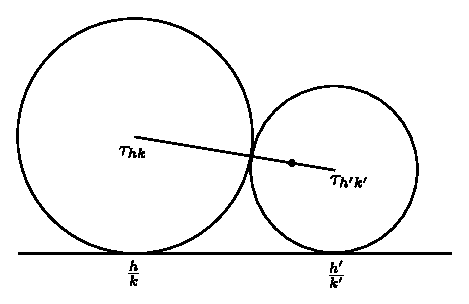
\includegraphics{vol2-figures/fig2.25.eps}}
\end{figure}

\noindent and\pageoriginale this, since 
\begin{align*}
  \frac{h}{k}< \frac{h'}{k'} ~\text{and}~ 
  \begin{vmatrix}h' & h\\ k'&k \end{vmatrix}=1, ~\text{is} & =
  \frac{h}{k} + \frac{k'}{k(k^2 + k'^2)} + \frac{i}{k^2 + k^{'2}}\\
  & = \frac{h}{k} + \xi'_{hk}
\end{align*}
where $\zeta'_{hk}= \dfrac{k'}{k(k^2+ k'^2)} + \dfrac{i}{k^2 +k'^2}$. We
notice that the imaginary part $1/(k^2+k'^2)$ gets smaller and smaller
as $k+ h'$ lies between $N$ and $2N$. Each arc runs from $\frac{h}{k}
+ \zeta'_{hk}$ to $\dfrac{h}{k} + \zeta''_{hk}$. Such an arc is the arc
$\nu_{hk}$. No arc touches the real axis.

We continue our study of the integral. Choose a number $N$, the order
of the Farey series, and cut the path of integration $P_N$ into pieces
$\gamma_{hk}$. 
\begin{align*}
  p(n) & = \int\limits_{P_N} f(e^{2 \pi i \tau}) e^{- 2 \pi i n \tau} d \tau\\
  & = \sum_{\substack{(h, k)=1\\ 0 \leq h < k \leq N}}
  \int\limits_{\gamma_{hk}} f(e^{2 \pi i \tau}) e^{- 2 \pi i n \tau} d \tau
\end{align*}

Now utilise the points of contact: put
\begin{align*}
\tau & = \frac{h}{k} + \zeta;\\
p(n) & = \sum_{\substack{(h, k)=1\\ 0 \leq h < k \leq N}}~
\int\limits^{\zeta''_{hk}}_{\zeta'_{hk}} f(e^{2 \pi i (\frac{h}{k}+ \zeta)}) e^{- 2 \pi i
  n (\frac{h}{k} + S)}dS
\end{align*}
($\gamma_{hk}$\pageoriginale goes from $\frac{h}{k} + \zeta'_{hk}$ to $\frac{h}{k} +
\zeta''_{hk}$; these are all arcs of radii $1/2k^2$). We make a further
substitution: put $\zeta= \dfrac{i z}{k^2}$, so that we turn round and
have everything in the right half-plane, instead of the upper
half-plane. (All these are only preparatory changes; there is no
actual mathematical progress as yet). Then
$$
p(n) = i \sum_{\substack{(h, k)=1\\ 0 \leq h < k \leq N}} \frac{e^{- 2
    \pi i n h/k}}{k^2}
  \int\limits^{\mathfrak{z}''_{hk}}_{\mathfrak{z}'_{hk}} f(e^{2 \pi i
    (\frac{h}{k} + \frac{i \mathfrak{z}}{k^2})}) e^{2 \pi n
    \mathfrak{z}/k^2} d \mathfrak{z}
$$

Now find out $\mathfrak{z}'_{hk}$ and $\mathfrak{z}''_{hk}$.
\begin{align*}
  \mathfrak{z}'_{hk} & = \frac{k^2 + i k k'}{k^2+ k'^2}\\
  \mathfrak{z}''_{hk} & = \frac{k^2 - i k k''}{k^2 + k''^2}
\end{align*}

So\pageoriginale what we have achieved so for is to cut the integral into
pieces.

\medskip
\noindent
\begin{minipage}{4.5cm}
 The whole thing lies on the right half-plane. The original
point of contact is 0 and everything lies on the circle
$|\mathfrak{z}- \dfrac{1}{2}| = \dfrac{1}{2}$. This is a
normalisation. We now study the complicated function on each arc
separately. We shall find that it is \textit{practically} the function
$\eta(\tau)$  about which we know a good deal:
$$
\eta \left( \frac{a \tau +b}{c \tau+d} \right)= \epsilon \sqrt{\frac{c \tau
  +d}{i}} \eta ( \tau), 
$$
\end{minipage}
\begin{minipage}{5.5cm}
\begin{figure}[H]
  \centering{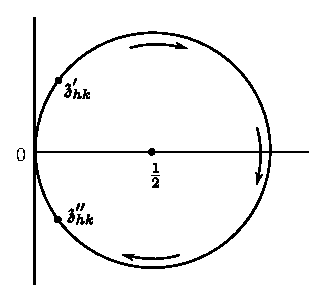
\includegraphics{vol2-figures/fig2.26.eps}}
\end{figure}
\end{minipage}
$\epsilon$ being a complicated 24th root of unity.
